\documentclass[aspectratio=169,11pt]{beamer}

% Shared style (ib-tutorials.sty at the repo root).
\makeatletter\def\input@path{{./}{../}}\makeatother
\usepackage{ib-tutorials}

\usepackage[utf8]{inputenc}
\usepackage{amsmath,amssymb}
\usepackage{booktabs}
\usepackage{array}
\newcolumntype{L}[1]{>{\raggedright\arraybackslash}p{#1}}
\usepackage{graphicx}
\graphicspath{{../pictures/3-ibamr-fundamentals/}{pictures/3-ibamr-fundamentals/}}
\usepackage{xcolor}
\usepackage{listings}
\usepackage{tikz}
\usetikzlibrary{arrows.meta,positioning,shapes.geometric,fit,calc}
\usepackage{hyperref}

\newcommand{\sourcecredit}[1]{\vfill\hfill{\tiny\textcolor{DarkGray}{#1}}}

\lstset{
  basicstyle=\ttfamily\scriptsize\color{BlackGray},
  keywordstyle=\color{NavyBlue}\bfseries,
  commentstyle=\color{DarkGray}\itshape,
  stringstyle=\color{OliveGreen},
  showstringspaces=false,
  columns=fullflexible,
  keepspaces=true,
  breaklines=true,
  breakindent=1em,
  frame=single,
  framerule=0.4pt,
  rulecolor=\color{LightGray},
  backgroundcolor=\color{LightGray!30},
  xleftmargin=0.25em,
  xrightmargin=0.25em
}
\lstdefinestyle{shell}{morecomment=[l]{\#}}
\lstdefinestyle{input}{morecomment=[l]{//}}
\lstdefinestyle{matlab}{morecomment=[l]{\%}}
\lstdefinestyle{python}{morecomment=[l]{\#}}
\lstdefinestyle{data}{}
\lstdefinestyle{tiny}{basicstyle=\ttfamily\tiny\color{BlackGray}}
\lstdefinestyle{inputtiny}{morecomment=[l]{//},basicstyle=\ttfamily\tiny\color{BlackGray}}
\lstdefinestyle{pythontiny}{morecomment=[l]{\#},basicstyle=\ttfamily\tiny\color{BlackGray}}

\title[Changing physical parameters wisely]{Changing physical parameters wisely}
\subtitle{Viscosity, density, speed, size and stiffness: what each one does, how to estimate the stiffnesses, and what else to change with them}
\author[Miller]{Laura A. Miller}
\institute[UArizona]{Department of Mathematics, University of Arizona}
\date{Using IB Software \textbullet\ Part III \textbullet\ Chapter 8a}

\begin{document}

% 1
\begin{frame}[plain]
\maketutorialtitlepanel{%
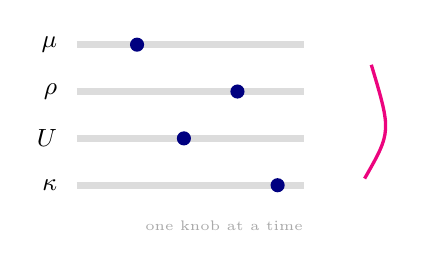
\begin{tikzpicture}[scale=0.85]
  \foreach \y/\lab/\pos in {2.2/$\mu$/0.9, 1.5/$\rho$/2.4, 0.8/$U$/1.6, 0.1/$\kappa$/3.0}{
    \draw[LightGray!80,line width=2.5pt] (0,\y) -- (3.4,\y);
    \fill[NavyBlue] (\pos,\y) circle (3pt);
    \node[font=\small,anchor=east] at (-0.15,\y) {\lab};}
  \draw[RubineRed,very thick] (4.3,0.2) .. controls (4.7,0.9) .. (4.4,1.9);
  \node[font=\tiny,text=DarkGray] at (2.2,-0.5) {one knob at a time};
\end{tikzpicture}}
\end{frame}

% 2
\begin{frame}{Learning goals}
\label{fr:goals}
\small By the end of this chapter you should be able to:
\begin{enumerate}
  \item find every physical parameter of a simulation: the ones at the top of the input file, the ones baked into the structure files by the generator, and the ones hidden in the boundary blocks and in \code{main.cpp};
  \item say what changes when you change one of them (viscosity, density, speed, size, stiffness), and what else must change with it (the time step, the structure spacing, the run length);
  \item estimate a spring, target or beam stiffness from the forces in the flow, and a damping coefficient, and say how rough those estimates are;
  \item read the Reynolds number of an example from its input file and know why the method is easiest near $\mathrm{Re} \approx 1$;
  \item change a parameter in an example, run a sweep, and recognize the mistakes that make a changed run meaningless.
\end{enumerate}
\begin{punchbox}
\small This chapter is the practical half of the old ``Changing physical parameters wisely'' lecture; the dimensionless analysis that justifies the estimates is chapter 8b. The two were one lecture in 2015 and are split here as the 2017 course split them.
\end{punchbox}
\end{frame}

% 3
\begin{frame}{How this chapter was checked}
\label{fr:checked}
\begin{itemize}
  \item The parameter values quoted are read from the input files, generators and READMEs of the 13 examples in this series (IB/01--08, IBFE/01--12), as shipped on the \code{master-tutorial} branch.
  \item The estimate formulas of the 2015--2018 slides are re-derived with their units on slides \ref{fr:kspring}--\ref{fr:kbeam2}; where a 2D and a 3D version were mixed up in the old slides, both are given and the mix-up is named.
  \item The viscosity and stiffness figures are new runs of IB/01 and IB/03 with IBAMR 0.19.0 (scripts in the references), analysed from the \code{hier\_data} position files with a short Python script that chapter 11 explains.
  \item The ``what can go wrong'' entries that are not from the course notes were produced on purpose and the symptoms are described from the runs.
\end{itemize}
\vspace{2mm}
\begin{punchbox}
\small Slide numbers refer to this deck; chapter numbers (5, 6, 7, 8b, 9a, 10, 11, 16) to the other chapters of Part III.
\end{punchbox}
\end{frame}

% 4
\begin{frame}{Where the parameters live}
\label{fr:where}
\scriptsize
\begin{tabular}{@{}L{0.22\textwidth}L{0.42\textwidth}L{0.26\textwidth}@{}}
\toprule
Place & What is there & To change it\\
\midrule
the top of \code{input2d}/\code{input3d} & \code{L}, \code{MU}, \code{RHO}, the speed (\code{V}, \code{U\_FLOW}), sometimes \code{Re}; the grid (\code{N}, \code{MAX\_LEVELS}), \code{DT}, \code{END\_TIME}; the IBFE material constants (\code{SHEAR\_MODULUS}, \code{KAPPA\_S}) & edit the line; no rebuild\\
the \code{VelocityBcCoefs} blocks & the boundary speeds and profiles, as block constants (chapter 7) & edit the block; no rebuild\\
the generator (\code{generate\_mesh2d.m}/\code{.py}) & the structure's size, point spacing $\Delta s$ and the stiffnesses $K$, $EI$, $\kappa$, which it writes into the files divided by $\Delta s$ (chapter 6) & edit, re-run the generator, new structure files\\
the structure files themselves & the per-element stiffnesses and rest lengths & regenerate (or the \code{uniform\_*} keys of chapter 6)\\
\code{main.cpp} & occasionally a hard-coded constant: a target-point velocity, a tether law, an IBFE stress law (chapters 9a, 15) & edit and rebuild\\
\bottomrule
\end{tabular}

\vspace{2mm}
\small The examples in this series were edited so that each physical quantity is set in \emph{one} place: the stream speed is \code{V} at the top of IB/03's input (the course version had \code{0.1} written into four boundary lines), the stiffnesses are variables at the top of the generators, and IB/08's viscosity can be set from a Reynolds number (slide \ref{fr:refrom}).
\end{frame}

% 5
\begin{frame}[fragile]{The physical parameters at the top of the input file}
\label{fr:top}
\begin{columns}[T,onlytextwidth]
\begin{column}{0.5\textwidth}
\small From the 2013--2018 slides: ``The physical parameters are given at the top of \code{input2d}. The immersed boundary works best when all terms are balanced ($\mathrm{Re} = 1$). Things get harder for $\mathrm{Re} < 0.001$ or $\mathrm{Re} > 1000$. Make sure your choices make sense: imagine what this thing would be in reality. You will likely need to change spring and beam stiffnesses. Think about how the forces are changing as you change parameters.''
\begin{lstlisting}[style=input]
// physical parameters
L = 1.0        // length of the computational (fluid) domain (m)
MU = 1.0e-1    // fluid dynamic viscosity (N s / m^2)
RHO = 1000     // fluid mass density (kg / m^3)
\end{lstlisting}
\end{column}
\begin{column}{0.48\textwidth}
\small Three numbers, and they set everything about the fluid:
\begin{itemize}
  \item \code{RHO}, the density $\rho$: inertia, and the scale of the pressure, $\rho U^2$;
  \item \code{MU}, the dynamic viscosity $\mu$: the viscous stress $\mu U/L$ and the viscous time $\rho L^2/\mu$;
  \item \code{L}, the box size: with \code{N} it fixes $\Delta x$ (chapter 7), and through the generator the point spacing.
\end{itemize}
The 2013 slide's \code{MU = 1.0e-1} is water-like for a decimetre-scale body at $0.1$ m/s; the examples in this series use $\mu = 100$ (IB/01, 02, 04, 06, 07), $4$ (IB/03), $40$ (IB/08) and $0.01$ with $\rho = 1$ (the IBFE set): slide \ref{fr:table}.
\end{column}
\end{columns}
\end{frame}

% 6
\begin{frame}{``Imagine what this thing would be in reality'': units}
\label{fr:units}
\small IBAMR has no units. Whatever system the input file uses is the system of the results, and the only check is yours.
\begin{itemize}
  \item The \al{IB examples} are in SI: a $1$ m box, water's density $1000$ kg/m$^3$, a viscosity of $4$ to $100$ N s/m$^2$ (water is $0.001$: these are syrup-to-honey fluids, chosen so that a decimetre-scale structure at $0.1$ m/s has $\mathrm{Re}$ of order 1, slide \ref{fr:re}), speeds of $0.1$ m/s, times in seconds.
  \item The \al{IBFE examples} are dimensionless: $\rho = 1$, $\mu = 0.01$, a box of side 2 or 16, speeds of $0.1$ to $1$. Their $\mu$ is $1/\mathrm{Re}$ for a unit speed and a unit length; IBFE/10 writes it so (\code{MU = 1.0/Re}).
  \item A stiffness copied from one set into the other is meaningless: $K = 2000$ in SI for a rubber band in syrup is not $K = 2000$ in a $\rho = 1$ world.
\end{itemize}
\vspace{1mm}
\begin{punchbox}
\small The test: write the problem down in words with units. ``A 20 cm rubber band in a fluid a hundred thousand times more viscous than water, relaxing from a 20\% stretch in about a second.'' If you cannot, the parameters are not yet chosen; if you can, the Reynolds number and the stiffness estimates follow (slides \ref{fr:re}, \ref{fr:kspring}).
\end{punchbox}
\vspace{1mm}
\small Chapter 8b does the same with dimensionless groups, so that one run stands for every physical case with the same $\mathrm{Re}$, $k'$ and $\mathrm{St}$.
\end{frame}

% 7
\begin{frame}[fragile]{Reminder from chapter 7: the domain, the grid and the time step}
\label{fr:reminder}
\small The 2013 and 2017 lectures opened with the domain and grid slides before the parameters; they are chapter 7 here, and this slide is the reminder.
\begin{columns}[T,onlytextwidth]
\begin{column}{0.5\textwidth}
\begin{lstlisting}[style=inputtiny]
CartesianGeometry {
   domain_boxes = [ (0,0) , (N - 1,N - 1) ]
   x_lo = -0.5*L, -0.5*L   // lower end of computational domain.
   x_up =  0.5*L,  0.5*L   // upper end of computational domain.
   periodic_dimension = 1, 1   // "overrides everything"
}
MAX_LEVELS = 4            // "4 is a good default"
REF_RATIO  = 4            // "a rather strict refinement ratio"
N = 8
NFINEST = (REF_RATIO^(MAX_LEVELS - 1))*N   // 512
DX = (1.0*L)/NFINEST
DT = 3.125e-2/NFINEST     // the 2013 guess; see chapter 7
\end{lstlisting}
\end{column}
\begin{column}{0.48\textwidth}
\footnotesize
\begin{itemize}
  \item ``As you start changing domain size, spatial step size, etc., you need to take care that everything still makes sense'' (2013). Change \code{x\_lo}/\code{x\_up} and \code{domain\_boxes} together; keep the cells square; coarsest counts $\ge 4$.
  \item \code{L} and \code{N} set $\Delta x$, and the generators set the point spacing from the same $N$: change one and re-run the other (slide \ref{fr:size}).
  \item The \code{DT} line is a CFL-type guess; the examples set it by hand from the stiffness (slide \ref{fr:dtstiff}).
\end{itemize}
\end{column}
\end{columns}
\end{frame}

% 8
\begin{frame}[fragile]{Reminder from chapter 7: outputs, end time, vorticity tagging}
\label{fr:reminder2}
\begin{columns}[T,onlytextwidth]
\begin{column}{0.5\textwidth}
\begin{lstlisting}[style=inputtiny]
// visualization dump parameters
   viz_writer = "VisIt"
   viz_dump_interval = 4000            // steps, not a count; 0 turns it off
   viz_dump_dirname = "viz_IB2d"
   visit_number_procs_per_file = 1
// hierarchy data dump parameters
   data_dump_interval = 1000           // steps
   data_dump_dirname = "hier_data_IB2d"   // the 2017 slide wrote _IB3d in a 2D file
IBStaggeredHierarchyIntegrator {       // 2013 name; now IBHierarchyIntegrator
   start_time = 0.0e0
   end_time   = 1.0e2                  // "another way to fill up the hard drive"
   grow_dt    = 1.1e0
   max_integrator_steps = 10000000
}
   using_vorticity_tagging = TRUE      // "too small tags the whole domain,
   vorticity_abs_thresh = 0.25         //  too big misses the wake"
\end{lstlisting}
\end{column}
\begin{column}{0.48\textwidth}
\scriptsize Why they matter for \emph{parameter} changes:
\begin{itemize}
  \item the intervals are in \al{steps}: when a new stiffness forces a smaller \code{DT}, the same interval writes more frames per second of simulated time. The series' inputs compute the interval from \code{END\_TIME} and \code{DT} (fifty frames per run) so this takes care of itself;
  \item \code{end\_time} must cover the \al{slowest} process of the new run: a more viscous fluid relaxes more slowly (slide \ref{fr:musweep}), a softer structure swings longer;
  \item a higher Reynolds number makes a longer wake: the vorticity threshold that followed the old wake may miss the new one.
\end{itemize}
\scriptsize The block name \code{IBStaggeredHierarchyIntegrator} is from the 2013 IBAMR; today the time integrator block is \code{IBHierarchyIntegrator} (or \code{IBExplicitHierarchyIntegrator}) and the fluid block \code{INSStaggeredHierarchyIntegrator} (chapter 3).
\end{column}
\end{columns}
\end{frame}

% 9
\begin{frame}{The examples' parameters: the IB set}
\label{fr:table}
\tiny
\setlength{\tabcolsep}{2pt}
\begin{tabular}{@{}L{0.13\textwidth}ccL{0.1\textwidth}L{0.17\textwidth}L{0.18\textwidth}cc@{}}
\toprule
example & $\mu$ & $\rho$ & speed & structure stiffness (generator) & in the file & \code{DT} & \code{END\_TIME}\\
\midrule
IB/01 rubber band & 100 & 1000 & its own & $K = 2000$ & $K/\Delta s = 2.04\times10^6$ & $10^{-4}$ & 2\\
IB/02 pulsatile channel & 100 & 1000 & 0--1 (pulse) & targets $\kappa = 10^4$; springs, beams $10^{-10}$ & $\kappa/\Delta s = 2.048\times10^6$ & $10^{-4}$ & 2\\
IB/03 tethered leaf & 4 & 1000 & 0.1 & $K = 30$, $EI = 5\times10^{-3}$, $\kappa = 30$ & $3.06\times10^4$, $5.31\times10^6$, $3.06\times10^4$ & $10^{-4}$ & 2\\
IB/04 moving cylinders & 100 & 1000 & prescribed path & targets $\kappa$ written directly & $4.096\times10^6$ & $2\times10^{-5}$ & 0.2\\
IB/06 growing springs & 100 & 1000 & its own & $K = 2000$, rest length grows & $2.04\times10^6$ & $10^{-4}$ & 0.5\\
IB/07 moving plates & 100 & 1000 & prescribed path & $K = 2000$, $EI = 5\times10^{-3}$, $\kappa = 2000$ & $2.04\times10^6$, $5.31\times10^6$, $2.04\times10^6$ & $10^{-4}$ & 1\\
IB/08 glycocalyx (3D) & 40 & 1000 & lid 0.1 & targets $\kappa = 5$ & $\kappa/\Delta s = 3.19\times10^4$ & $10^{-5}$ & 0.2\\
\bottomrule
\end{tabular}

\vspace{2mm}
\small All boxes are $1$ m (IB/02: $5$ m; IB/08: $\frac18\times\frac18\times1$ m), all finest grids $512$ cells per metre (IB/04: $1024$), all point spacings about $\Delta x/2$. The file values are the generator's stiffness divided by $\Delta s$ (springs, targets) or $\Delta s^3$ (beams): chapter 6. ``Its own'' speed means nothing is imposed: the structure moves because it is stretched or because its rest lengths change.
\end{frame}

% 10
\begin{frame}{The examples' parameters: the IBFE set}
\label{fr:table2}
\scriptsize
\setlength{\tabcolsep}{3pt}
\begin{tabular}{@{}L{0.2\textwidth}cccL{0.3\textwidth}cc@{}}
\toprule
example & $\mu$ & $\rho$ & speed & solid & \code{DT} & \code{END\_TIME}\\
\midrule
IBFE/01 tethered plate & 0.01 & 1 & tether 0.5 & neo-Hookean, $\mu_s = 10$; tether $\kappa = 10^6$ & $10^{-3}$ & 4\\
IBFE/05 gmsh triangle & 0.01 & 1 & tether 0.5 & same material and tether & $5\times10^{-4}$ & 4\\
IBFE/06 active tension & 0.01 & 1 & its own & $\mu_s = 10$ plus an active stress & $10^{-3}$ & 4\\
IBFE/08 plate hits circle & 0.01 & 1 & tether 0.25 & $\mu_s = 10$ both parts; tether $10^6$ & $5\times10^{-4}$ & 4\\
IBFE/10 flow tank (3D) & $1/\mathrm{Re} = 0.01$ & 1 & stream 0.1 & compressible neo-Hookean, $\nu = 0.3$; tether $10^5$ & $10^{-4}$ & 0.5\\
IBFE/12 advection--diffusion & 0.01 & 1 & tether 0.5 & IBFE/01's plate; scalar diffusivity $10^{-6}$ & $10^{-3}$ & 4\\
\bottomrule
\end{tabular}

\vspace{2mm}
\small Boxes of side 2 (IBFE/10: $32\times16\times16$), finest grids of $128$ cells (IBFE/10: $256$ per 16). The solid's stiffness is a \al{material constant} (the shear modulus $\mu_s$, in units of pressure) rather than a spring constant per point, so it does not scale with $\Delta s$; what scales with the mesh is the tether penalty $\kappa$, a force per unit volume per unit displacement (chapter 15). The time steps are ten times those of the IB set because the fluid is a thousand times lighter: slide \ref{fr:dtstiff}.
\end{frame}

% 11
\begin{frame}{The Reynolds number of an example}
\label{fr:re}
\small $\mathrm{Re} = \rho U L/\mu$: inertial over viscous forces. The number means nothing until $U$ and $L$ are named; the examples' READMEs name them.
\vspace{1mm}

\scriptsize
\begin{tabular}{@{}L{0.17\textwidth}L{0.28\textwidth}L{0.2\textwidth}L{0.25\textwidth}@{}}
\toprule
example & $U$ & $L$ & $\mathrm{Re}$\\
\midrule
IB/03 leaf & the stream, $0.1$ m/s & the leaf's length, $0.1$ m & $2.5$\\
IB/08 glycocalyx & the shear flow at the fibre's height, $Vh/L = 0.0156$ m/s & the fibre's height, $0.156$ m & $0.061$\\
IBFE/10 flow tank & the stream, $0.1$ & the plate's width, $2$ & $20$ (the input's \code{Re = 100} is for $U = L = 1$)\\
IB/01 rubber band & the band's own speed, about $0.02$ m/s as it rounds up & its diameter, $0.2$ m & about $0.04$\\
IB/02 channel & the peak, $1$ m/s & the channel width, $1$ m & $10$ (and a Womersley number of $8.9$, chapter 7)\\
IBFE/01 plate & the tether's speed, $0.5$ & the plate's length, $1$ & $50$\\
\bottomrule
\end{tabular}

\vspace{2mm}
\small So the series runs from creeping flow (IB/01, IB/08) through $\mathrm{Re} \sim 1$ (IB/03) to the tens (IB/02, IBFE/01, IBFE/10): all within the band where the 2013 slide says the method is comfortable. None is above $1000$. Chapter 8b has the dimensionless numbers that go with $\mathrm{Re}$ (Strouhal, Womersley, P\'eclet) and the biological ranges.
\end{frame}

% 12
\begin{frame}{Why the method is easiest near $\mathrm{Re} \approx 1$}
\label{fr:re2}
\small The 2013 statement, ``the immersed boundary works best when all terms are balanced ($\mathrm{Re} = 1$); things get harder for $\mathrm{Re} < 0.001$ or $\mathrm{Re} > 1000$'', is a rule of thumb. The reasons behind it:
\begin{itemize}
  \item \al{Low $\mathrm{Re}$} (creeping flow): nothing is wrong with the fluid solve (the viscous term is implicit), but the structure must be \emph{stiff} relative to the viscous forces to hold its shape, and a stiff structure means a small time step (slide \ref{fr:dtstiff}); the viscous time $\rho L^2/\mu$ is short, so transients die at once, but any motion you impose is resisted by large forces that the explicit coupling must survive. At $\mathrm{Re} \ll 10^{-3}$ one is better off with a Stokes solver and a different method.
  \item \al{High $\mathrm{Re}$}: boundary layers of thickness $\delta \sim L/\sqrt{\mathrm{Re}}$ must be resolved by the grid, while the IB kernel smears the interface over about four cells (chapter 5); when $\delta$ falls below a few $\Delta x$ the forces on the body are wrong. The wake carries vorticity far downstream (vorticity tagging, bigger boxes, chapter 7), and in 3D the flow becomes turbulent. Above $\mathrm{Re} \sim 1000$ the cost grows fast and the thin-interface assumption weakens.
  \item \al{Near $1$}: viscous and inertial forces are comparable, both are resolved by the same grid, the structure forces are moderate, and the time step is set by the structure alone.
\end{itemize}
\vspace{1mm}
\small Biology spends most of its time in this comfortable band: small swimmers, cilia and flagella (low), larvae, jellyfish, insect wings (1--1000); chapter 8b's chart.
\end{frame}

% 13
\begin{frame}{Change one parameter, and what changes with it}
\label{fr:propagate}
\scriptsize
\setlength{\tabcolsep}{3pt}
\begin{tabular}{@{}L{0.14\textwidth}L{0.36\textwidth}L{0.42\textwidth}@{}}
\toprule
You change & what changes in the physics & what you must change with it\\
\midrule
$\mu$ (\code{MU}) & $\mathrm{Re} \propto 1/\mu$; the viscous time $\rho L^2/\mu$; viscous forces on the structure $\propto \mu$ (at low $\mathrm{Re}$) & \code{END\_TIME} (slower relaxation at high $\mu$, slide \ref{fr:musweep}); stiffnesses, if the structure must hold against the larger forces; \code{DT} only indirectly (slide \ref{fr:dtstiff})\\
$\rho$ (\code{RHO}) & $\mathrm{Re} \propto \rho$; inertia; the pressure scale $\rho U^2$; the added mass felt by the structure & the stiffnesses that were estimated from $\rho U^2$; \code{DT}: the stable step of an explicit IB coupling scales with $\sqrt{\rho}$ (the IBFE set at $\rho = 1$ runs ten times the step of the IB set at $1000$)\\
$U$ (\code{V}, \code{U\_FLOW}) & $\mathrm{Re} \propto U$; forces $\propto U^2$ ($\mathrm{Re} > 1$) or $U$ ($\mathrm{Re} < 1$); the CFL number $U\Delta t/\Delta x$; the time to cross the box $L/U$ & \code{DT} if the CFL limit is approached (rare for the IB set, slide \ref{fr:dtstiff}); stiffnesses (slide \ref{fr:kspring}); \code{END\_TIME} (more or fewer cycles)\\
$L$ or $N$ & $\Delta x = L/N$; the point spacing $\Delta s \approx \Delta x/2$; the resolution of the structure & \al{re-run the generator} (slide \ref{fr:size}); the file stiffnesses change with $\Delta s$ automatically when you do; \code{DT} if $\Delta x$ shrinks\\
a stiffness ($K$, $EI$, $\kappa$) & how far the structure deforms or strays from its target & \code{DT}: halve it when you multiply a stiffness by four (slide \ref{fr:dtstiff}); nothing else\\
\bottomrule
\end{tabular}

\vspace{2mm}
\small ``Think about how the forces are changing as you change parameters'' (2013): every row above is a force balance. The next slides show two rows in runs: viscosity on the rubber band, stiffness on the leaf.
\end{frame}

% 14
\begin{frame}{Viscosity: the rubber band at $\mu = 100$, $10$ and $1$}
\label{fr:musweep}
\begin{columns}[T,onlytextwidth]
\begin{column}{0.56\textwidth}
\centering
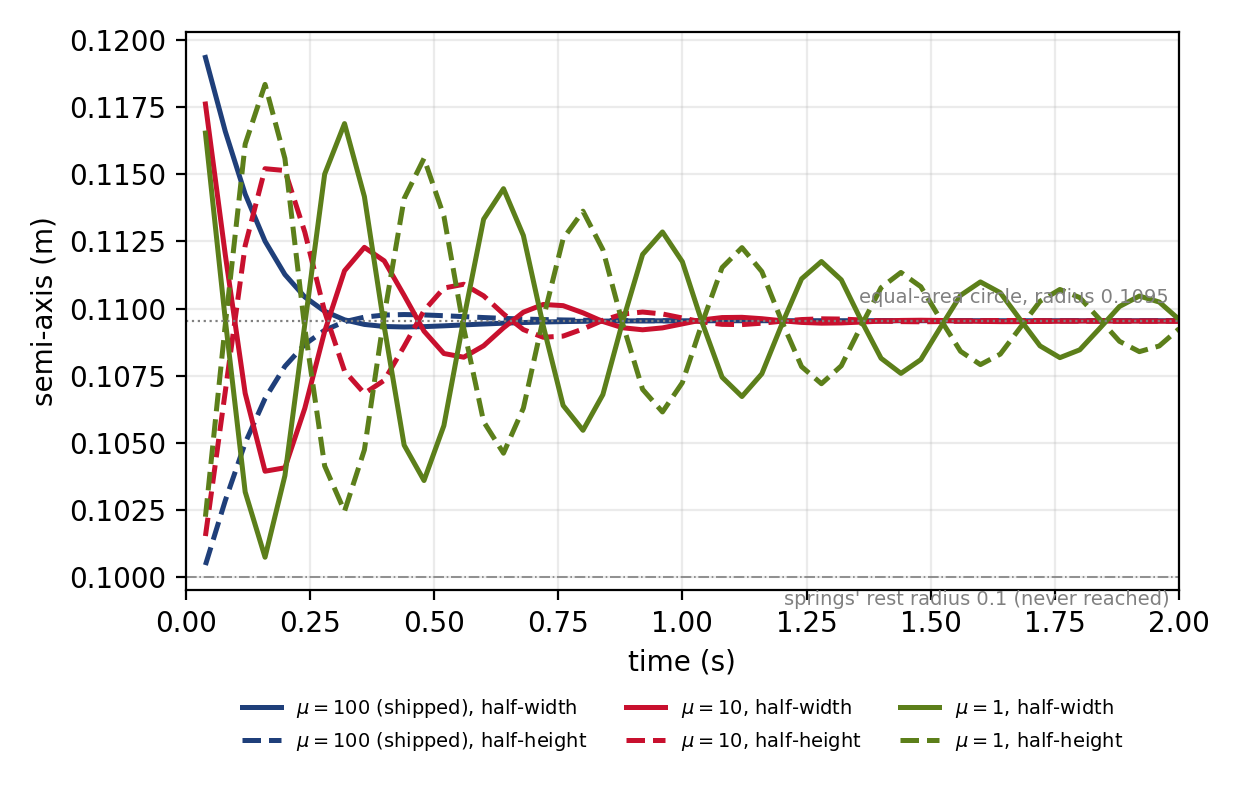
\includegraphics[width=\textwidth]{ch8a-band-mu-axes}
\end{column}
\begin{column}{0.42\textwidth}
\scriptsize IB/01's band starts as an ellipse ($0.12 \times 0.10$ m) and its springs pull it toward a circle of radius $0.1$ m. Three runs differ only in \code{MU}:
\begin{itemize}
  \item $\mu = 100$ (shipped): \al{overdamped}; the semi-axes creep together, within 2 mm of each other by $t = 0.24$ s, and never cross;
  \item $\mu = 10$: \al{underdamped}; the band overshoots (half-width down to $0.104$ m at $t = 0.16$ s, taller than wide) and swings with a period of $0.37$ s, each swing smaller than the last;
  \item $\mu = 1$: a deeper overshoot ($0.101$ m) and a period of $0.32$ s, with little decay over the 2 s.
\end{itemize}
\scriptsize The spring constant is the same in all three; only the fluid's resistance changed. The curves are the band's half-width (solid) and half-height (dashed) from the \code{X.*} position files, written every $0.04$ s.
\end{column}
\end{columns}
\sourcecredit{IB/01 with IBAMR 0.19.0, \code{MU} = 100, 10, 1, everything else as shipped (\code{wsl/final/run\_ch8a\_ib01.sh}); semi-axes computed by \code{tools/ch8a\_figures.py} from \code{hier\_data\_IB2d/X.*}.}
\end{frame}

% 14b
\begin{frame}{Why the band settles at $0.1095$ m, not at its rest radius}
\label{fr:musweep1b}
\small All three runs end on the same circle, of radius $0.1095$ m, and none reaches the springs' rest radius of $0.1$ m.
\begin{itemize}\footnotesize
  \item The fluid inside the band is \al{incompressible} and the band is closed, so the enclosed area cannot change: the ellipse with semi-axes $0.12$ and $0.10$ m becomes the circle with the same area, $\pi\,(0.12\times0.10) = \pi\,(0.1095)^2$.
  \item The springs therefore stay stretched by $9.5\%$, and their tension is balanced by a pressure inside the band that is higher than outside: a tension of $K \times 0.095$ per unit depth over a radius of $0.1095$ m gives, by Laplace's law, $\Delta p = T/R \approx 2000 \times 0.095/0.1095 \approx 1.7\times10^3$ N/m$^2$ at the end of every run.
  \item This is the IB method's \al{volume conservation} at work (chapter 5): a closed membrane in an incompressible fluid holds its area to the accuracy of the discrete divergence, which is why the three final radii agree to four digits ($0.1095$, $0.1095$, $0.1096$).
\end{itemize}
\vspace{1mm}
\begin{punchbox}
\small Two checks fall out of this for any closed structure: the final size is set by the enclosed area, not by the rest lengths, and a steady pressure jump across the membrane of $T/R$ should be visible in the \code{P} field in VisIt. If the band \emph{did} shrink to its rest radius, fluid would be leaking through it (points too far apart, chapter 5).
\end{punchbox}
\end{frame}

% 15
\begin{frame}{Viscosity: the band's shape at three times}
\label{fr:musweep2}
\centering
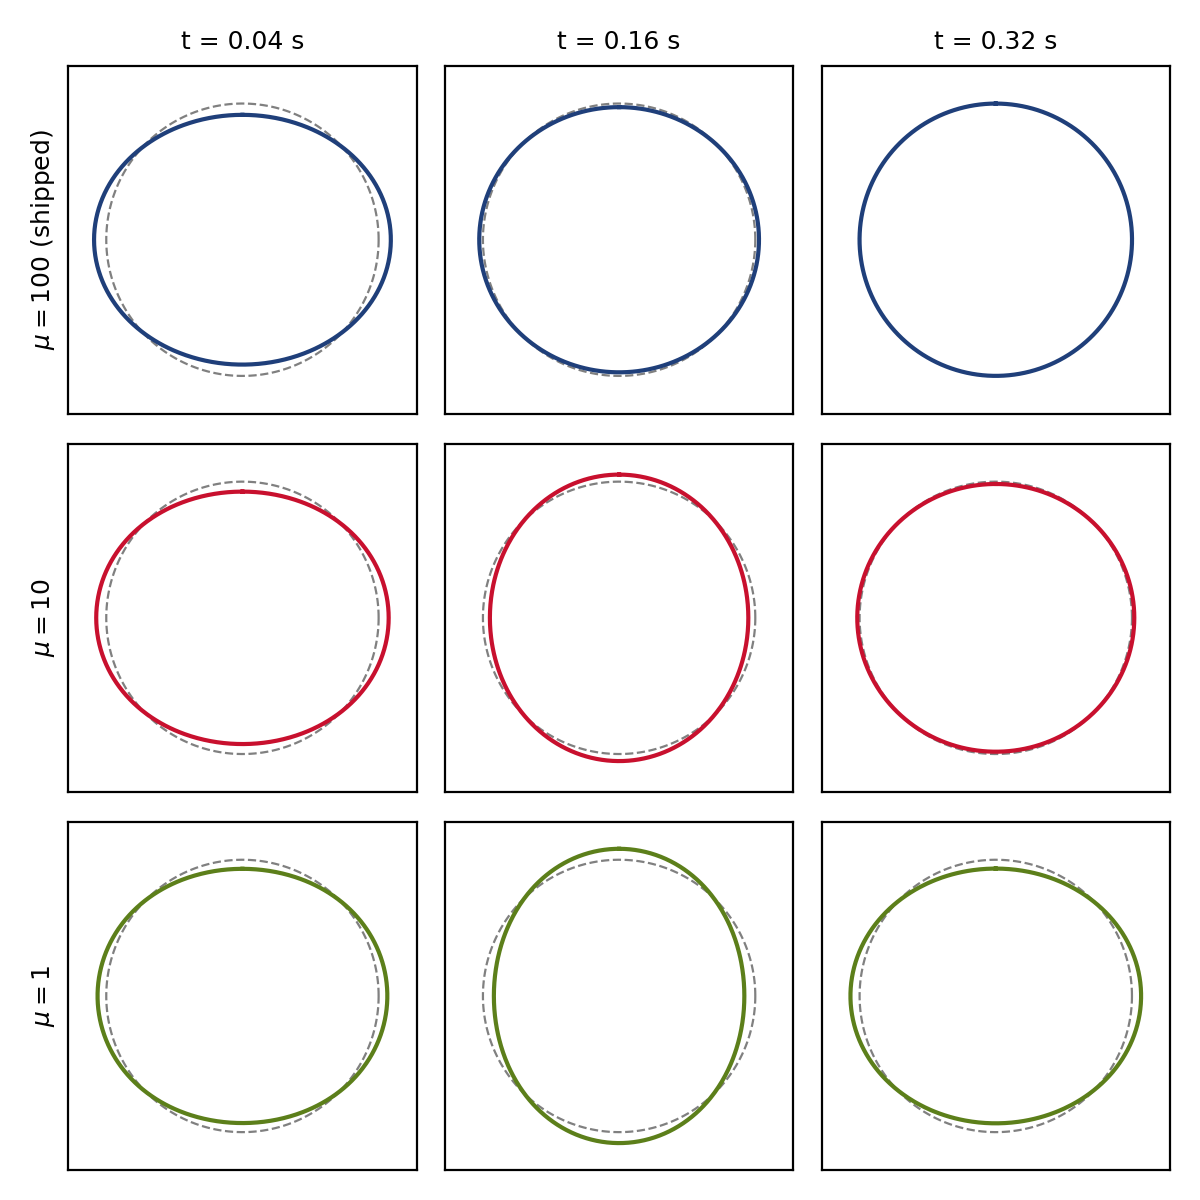
\includegraphics[height=0.6\textheight]{ch8a-band-mu-shapes}
\vspace{1mm}

\small Rows: $\mu = 100$, $10$, $1$; columns: three times during the run. The dashed circle is the final shape, the circle with the ellipse's area. At $\mu = 100$ the band is never far from an ellipse shrinking onto the circle; at $\mu = 10$ and $1$ it passes through the circle at about $t = 0.12$ s and comes out the other side, taller than wide, then swings back.
\sourcecredit{Same runs; outlines drawn from \code{X.*} by \code{tools/ch8a\_figures.py}.}
\end{frame}

% 16
\begin{frame}{What the viscosity sweep shows}
\label{fr:musweep3}
\small Two time scales compete in the band:
\begin{itemize}
  \item the \al{elastic} one: a ring of radius $R$ with tension stiffness $K$ (N/m per unit depth) moving the fluid it encloses, of mass $\sim \rho R^2$ per unit depth, has a time scale $\sqrt{\rho R^3/K} = \sqrt{1000 \times 0.0013/2000} \approx 0.026$ s, or $2\pi$ times that, $0.16$ s, for a period. The measured swing is $0.32$ s ($\mu = 1$) to $0.37$ s ($\mu = 10$): the right order, with a factor of two from the added mass outside the band and the shape of the mode;
  \item the \al{viscous} one: momentum diffuses across the band in $\rho R^2/\mu$, which is $0.12$ s at $\mu = 100$ (the fluid stops the band within a fraction of a period: overdamped), $1.2$ s at $\mu = 10$ (a few decaying swings), $12$ s at $\mu = 1$ (many swings with little decay, as the run shows).
\end{itemize}
\vspace{1mm}
\begin{punchbox}
\small \al{The rule in one line:} viscosity does not change what the structure wants to do, only how fast the fluid lets it, and whether it overshoots. A run that ``does nothing'' after a viscosity increase has not been run long enough: scale \code{END\_TIME} with $\mu$. A run that oscillates after a viscosity decrease is not unstable; it is underdamped. Instability looks different (chapter 16: growth without bound, then \code{Time step size change encountered}).
\end{punchbox}
\vspace{1mm}
\footnotesize The same three runs are IB/01's job-array sweep (\code{params.txt}: 100, 10, 1; chapter 3), so the figure can be reproduced on Puma with one \code{sbatch}.
\end{frame}

% 17
\begin{frame}{Stiffness: the leaf with the beam stiffness divided and multiplied by ten}
\label{fr:kbsweep}
\begin{columns}[T,onlytextwidth]
\begin{column}{0.56\textwidth}
\centering
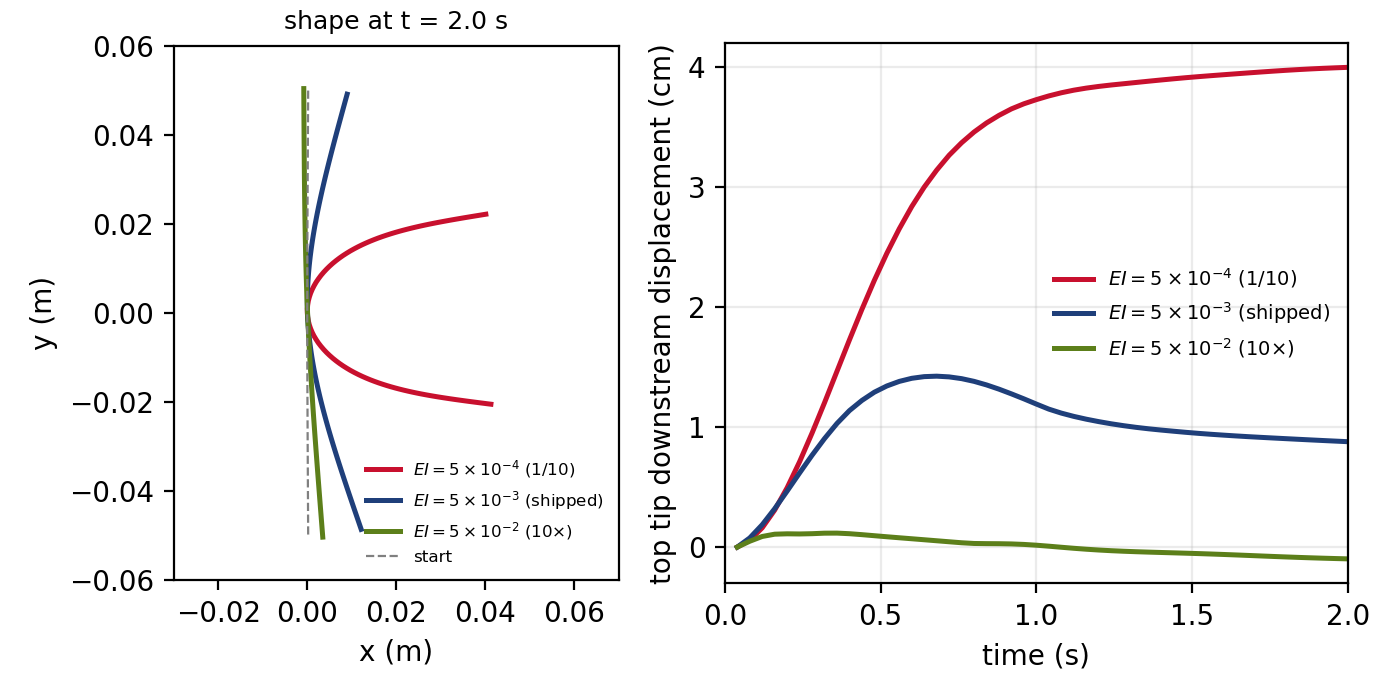
\includegraphics[width=0.96\textwidth]{ch8a-leaf-kbeam}
\end{column}
\begin{column}{0.42\textwidth}
\scriptsize IB/03's leaf in the same stream ($\mathrm{Re} = 2.5$) with three bending stiffnesses: $EI = 5\times10^{-4}$, the shipped $5\times10^{-3}$, and $5\times10^{-2}$. The structure files were regenerated with \code{kappa\_beam} changed in \code{generate\_mesh2d.py}; nothing else was touched except, for the stiff case, \code{DT} (next slide).
\begin{itemize}
  \item left: the leaf's shape at $t = 2$ s for the three runs, with the starting line dashed;
  \item right: the downstream displacement of the top tip against time.
\end{itemize}
\scriptsize The shipped leaf bends most at $t \approx 0.7$ s ($1.4$ cm) and relaxes to $0.9$ cm as the flow around it settles; the ten-times-softer leaf folds over, its tips $4$ cm downstream and pointing with the flow; the ten-times-stiffer one moves about a millimetre.
\end{column}
\end{columns}
\sourcecredit{IB/03 with IBAMR 0.19.0 (\code{wsl/final/run\_ch8a\_ib03.sh}, \code{run\_ch8a\_ib03b.sh}); shapes and tip positions from \code{X.*} by \code{tools/ch8a\_figures.py}. The shipped run is the one of chapters 6 and 7.}
\end{frame}

% 17b
\begin{frame}{What the stiffness sweep shows, and what it cost}
\label{fr:kbsweep2}
\footnotesize
\begin{itemize}
  \item The displacement is \al{not} proportional to $1/EI$: a tenth of the stiffness gave about three times the tip displacement at $t = 2$ s ($4.0$ cm against $0.9$), not ten. The bent leaf presents less area to the stream and lets it flow past, so the softer it is, the less force it feels. That is the fluid--structure coupling at work, and the reason the estimates of the next slides are only estimates: they assume the load of the undeformed shape.
  \item The shipped leaf's \al{overshoot} at $t \approx 0.7$ s is the stream's start-up: the tanh ramp (chapter 7) is still accelerating the fluid, and the leaf is pushed furthest while the flow around it is still developing; it springs back as the wake forms.
  \item The \al{stiff} leaf did not run at the shipped time step. With \code{kappa\_beam} ten times larger and \code{DT = 1e-4} unchanged, the run stopped at step 15 ($t = 0.0015$ s) with \code{IBHierarchyIntegrator::preprocessIntegrateHierarchy(): Time step size change encountered}: the explicit coupling could not take the stiffer beam's forces at that step, the integrator cut the step, and \code{error\_on\_dt\_change} turned the cut into an abort (chapter 5). With \code{DT = 2.5e-5}, a quarter, it ran to the end, four times slower.
\end{itemize}
\vspace{1mm}
\begin{punchbox}
\small So the sweep demonstrates both rows of slide \ref{fr:propagate} for a stiffness: the deformation changes less than linearly, and the time step must follow the stiffness, by roughly $1/\sqrt{\text{factor}}$ (slide \ref{fr:dtstiff}).
\end{punchbox}
\end{frame}

% 18
\begin{frame}{Estimating $k_{\mathrm{spring}}$ (and a target stiffness)}
\label{fr:kspring}
\small The 2017 recipe, kept word for word: ``By estimating the force acting on the boundary ($F_b$) and the desired displacement ($x_s$), one can make an educated guess for $k_{\mathrm{spring}}$. The idea is to set $k_{\mathrm{spring}} = F_b/x_s$. Choose $x_s$ to be the maximum desired displacement from the target point or the maximum amount of displacement from a resting length. The estimate for $F_b$ will depend on $\mathrm{Re}$ and dimension (dim). For the characteristic velocity, $U$, I recommend using $U_{\max}$.''
\[
  F_b \sim \tfrac12\,\rho\,\Delta x^{\,\mathrm{dim}-1}\,U^2 \quad (\mathrm{Re} > 1), \qquad
  F_b \sim \mu\,U\,\Delta x^{\,\mathrm{dim}-2} \quad (\mathrm{Re} < 1).
\]
``Warning to user: these are really rough estimates.''
\begin{itemize}
  \item[] \hspace{-4mm}$F_b$ is the force on \al{one point}, which represents a piece of boundary $\Delta x$ across (in 2D, per unit depth). At $\mathrm{Re} > 1$ it is the dynamic pressure $\frac12\rho U^2$ on that piece's area, $\Delta x^{\mathrm{dim}-1}$. At $\mathrm{Re} < 1$ it is a Stokes drag, viscosity times speed times a length: $\mu U \Delta x$ in 3D, $\mu U$ per unit depth in 2D.
  \item[] \hspace{-4mm}$k$ here is the stiffness \al{in the file}, the one that multiplies the displacement of that point: for a target point $\kappa/\Delta s$, for a spring $K/\Delta s$ (chapter 6).
\end{itemize}
\begin{punchbox}
\footnotesize \al{Correction.} The 2017 slide wrote the viscous case as $F_b \sim \mu\,\Delta x\,U$ for both dimensions. That is the 3D form; in 2D the $\Delta x$ drops out (units: $\mu U$ is already a force per unit depth), hence the $\Delta x^{\mathrm{dim}-2}$ above.
\end{punchbox}
\end{frame}

% 19
\begin{frame}{The estimate applied to the examples}
\label{fr:kspring2}
\scriptsize
\setlength{\tabcolsep}{3pt}\renewcommand{\arraystretch}{0.97}
\begin{tabular}{@{}L{0.16\textwidth}L{0.3\textwidth}L{0.14\textwidth}L{0.1\textwidth}L{0.2\textwidth}@{}}
\toprule
example (points) & $F_b$ on one point & $x_s$ & estimate & in the file\\
\midrule
IB/03 springs ($\mathrm{Re} = 2.5$, 2D) & $\frac12\rho\Delta x U^2 = \frac12\cdot1000\cdot\frac{1}{512}\cdot0.01 = 9.8\times10^{-3}$ & 10\% of $\Delta s$, $10^{-4}$ m & $\approx 10^2$ & $3.06\times10^4$ (300$\times$)\\
IB/02 targets ($\mathrm{Re} = 10$, 2D) & $\frac12\cdot1000\cdot\frac{5}{512}\cdot1 = 4.9$ & $0.1\,\Delta x = 10^{-3}$ m & $\approx 5\times10^3$ & $2.05\times10^6$ (400$\times$)\\
IB/08 targets ($\mathrm{Re} = 0.06$, 3D) & $\mu U \Delta x = 40\cdot0.0156\cdot\frac{1}{512} = 1.2\times10^{-3}$ & $0.1\,\Delta x = 2\times10^{-4}$ m & $\approx 6$ & $3.19\times10^4$ (5000$\times$)\\
IB/04 targets ($\mathrm{Re} \ll 1$, 2D) & $\mu U = 100\cdot U_{\mathrm{cyl}}$; with $U_{\mathrm{cyl}} \sim 0.1$: $10$ & $0.1\,\Delta x = 10^{-4}$ m & $\approx 10^5$ & $4.10\times10^6$ (40$\times$)\\
\bottomrule
\end{tabular}

\vspace{2mm}
\small Every example is far stiffer than the estimate, by a factor of 40 to 5000. That is deliberate:
\begin{itemize}
  \item the estimate is the stiffness at which the point moves by $x_s$ under the \emph{mean} load; a wall that must stay put against a pulsing flow, or a fibre that must be inextensible, wants ten to a hundred times more;
  \item the \al{price} is the time step: the file stiffness sets the stable \code{DT} (slide \ref{fr:dtstiff}), which is why IB/04, the stiffest, runs at $2\times10^{-5}$ s.
\end{itemize}
\small So use the estimate as a \al{floor}, multiply by 10--100 for a wall or a tether, and then pay for it in \code{DT}. If the structure still stretches or strays too far, the stiffness goes up again; if the run becomes unstable, \code{DT} goes down.
\end{frame}

% 20
\begin{frame}{Estimating $k_{\mathrm{beam}}$}
\label{fr:kbeam}
\small The 2015/2017 recipe: ``By using the dimensionless beam stiffness $k'_{\mathrm{beam}}$, one can make an educated guess for $k_{\mathrm{beam}}$. Setting $k'_{\mathrm{beam}} = 10$ typically results in a little bit of bending (maybe 2--10 degrees). $U$ is the characteristic velocity (try $U_{\max}$) and $L$ is the characteristic length. I would use the length of the boundary.''
\[
  \text{2D, } \mathrm{Re} > 1:\quad k'_{\mathrm{beam}} = \frac{k_{\mathrm{beam}}}{\rho U^2 L^3}; \qquad
  \text{2D, } \mathrm{Re} < 1:\quad k'_{\mathrm{beam}} = \frac{k_{\mathrm{beam}}}{\mu U L^2}; \qquad
  \text{3D:}\quad k'_{\mathrm{beam}} = \frac{EI}{\rho U^2 L^4}.
\]
\begin{itemize}
  \item $k_{\mathrm{beam}}$ is the \al{flexural rigidity}, $EI$ in 3D (N m$^2$) and $EI$ per unit depth in 2D (N m): the generator's \code{kappa\_beam}, not the file value, which is $k_{\mathrm{beam}}/\Delta s^3$ (chapter 6).
  \item The denominators are the fluid's bending moment scale: a pressure $\rho U^2$ (or a viscous stress $\mu U/L$) over a length $L$, times a lever arm $L$, times the width ($L$ again in 3D, unit depth in 2D).
\end{itemize}
\vspace{1mm}
\begin{punchbox}
\small \al{Correction.} The 2017 slide wrote $k'_{\mathrm{beam}} = k_{\mathrm{beam}}/(\rho U^2 L^4)$ under the heading ``in 2D''. $L^4$ is the 3D form (the 2015 and 2020 slides have $L^3$ for 2D); with $L^4$ the number is not dimensionless in 2D and is off by a factor $L$, which for a decimetre-scale body is a factor of ten.
\end{punchbox}
\end{frame}

% 21
\begin{frame}{The beam estimate applied to the leaf, and what the sweep says}
\label{fr:kbeam2}
\small IB/03: $k_{\mathrm{beam}} = 5\times10^{-3}$ N m, $\rho = 1000$, $U = 0.1$ m/s, $L = 0.1$ m (the leaf's length):
\[
  k'_{\mathrm{beam}} = \frac{5\times10^{-3}}{1000 \times 0.01 \times 10^{-3}} = 0.5 .
\]
\begin{itemize}
  \item So the shipped leaf is twenty times \emph{softer} than the ``$k' = 10$, a few degrees'' setting, and it bends accordingly: the top tip is $0.9$ to $1.4$ cm downstream on a leaf whose half-length is 5 cm, a chord angle of $10$--$16$ degrees from the vertical (slide \ref{fr:kbsweep}).
  \item The ten-times-stiffer run ($k' = 5$) bends about a degree, near the recipe's ``2--10 degrees at $k' = 10$'' for a stiffness twice the recipe's; the ten-times-softer run ($k' = 0.05$) folds over.
  \item At $\mathrm{Re} = 2.5$ the viscous form gives $k_{\mathrm{beam}}/(\mu U L^2) = 5\times10^{-3}/(4\times0.1\times0.01) = 1.25$: the same order, as it should be when $\mathrm{Re}$ is near 1.
\end{itemize}
\begin{punchbox}
\footnotesize \al{How to use it:} decide how much bending you want (a stiff fin: $k' \sim 10$; a flapping flag or a leaf in the wind: $k' \sim 0.1$--$1$; a filament that folds: $k' \ll 0.1$), compute $k_{\mathrm{beam}} = k'\,\rho U^2 L^3$ (2D), put it in the generator, and let chapter 10 refine it with the beam theory (the bending length and the Cauchy number). ``Warning to user: these are really rough estimates.''
\end{punchbox}
\end{frame}

% 22
\begin{frame}{The stiffnesses and their units, in one place}
\label{fr:unitsk}
\scriptsize
\setlength{\tabcolsep}{3pt}
\begin{tabular}{@{}L{0.15\textwidth}L{0.24\textwidth}L{0.2\textwidth}L{0.3\textwidth}@{}}
\toprule
element & generator constant & file value & force law (chapter 6)\\
\midrule
spring & $K$: tension per unit strain; N (3D) or N/m (2D, per depth) & $K/\Delta s$ & $(K/\Delta s)\,(|\mathbf{X}_j - \mathbf{X}_i| - r)$ along the spring\\
target point & $\kappa$: tether stiffness per unit length of boundary & $\kappa/\Delta s$ & $(\kappa/\Delta s)\,(\mathbf{X}_{\mathrm{target}} - \mathbf{X}) - \eta\,\mathbf{U}$\\
beam & $EI$: flexural rigidity; N m$^2$ (3D), N m (2D) & $EI/\Delta s^3$ & $-(EI/\Delta s^3)\,(\mathbf{X}_{i-1} - 2\mathbf{X}_i + \mathbf{X}_{i+1})$ on the triple\\
IBFE tether & $\kappa_s$ (\code{KAPPA\_S}): force per unit volume per unit displacement & as is & $\kappa_s\,(\mathbf{X}_0 - \mathbf{X})$ per unit reference volume\\
IBFE material & $\mu_s$ (\code{SHEAR\_MODULUS}): a pressure & as is & the stress law of the example (chapter 15)\\
\bottomrule
\end{tabular}

\vspace{2mm}
\small Two consequences for parameter changes:
\begin{itemize}
  \item the \al{file values depend on $\Delta s$}: refine the grid and the generator must be re-run so that $K/\Delta s$ and $EI/\Delta s^3$ are recomputed; copying the old files onto a finer grid makes the structure softer by the ratio of spacings (springs) or its cube (beams);
  \item the \al{estimates of slides \ref{fr:kspring}--\ref{fr:kbeam2} are for the file value} (spring, target) and for the generator constant (beam), because the point force uses the file value and the bending moment uses $EI$. Keep the two straight; the generators' comments say which is which.
\end{itemize}
\end{frame}

% 23
\begin{frame}{Estimating damping}
\label{fr:damping}
\footnotesize The 2017 recipe: ``The goal is to make the springs close to critically damped. This means setting the damping coefficient $c = 2\sqrt{k_{\mathrm{spring}}\,m}$. The hard part is estimating $m$. Recall the boundary is massless, but there is the added mass of the fluid. My recommendation is to try setting $m = \rho\,\Delta x^{\mathrm{dim}}$. Warning to user: these are really rough estimates.''
\begin{itemize}
  \item Where damping is available: IBAMR's \al{target points} take an optional damping coefficient $\eta$ as a third column of the \code{.target} file (or \code{uniform\_target\_damping}), which adds $-\eta\,\mathbf{U}$ to the tether force (chapter 6). Plain springs and beams have none; a damped spring is a custom force (chapter 9b). IB2d has damped springs as a file type (chapter 4a).
  \item $m = \rho\,\Delta x^{\mathrm{dim}}$ is the mass of the fluid in one cell: the fluid that the point drags with it, which is what resists a change of its velocity.
  \item Worked number, IB/02's walls: $k = 2.05\times10^6$ (file), $m = 1000 \times (5/512)^2 = 0.095$ kg per unit depth, so $c = 2\sqrt{2.05\times10^6 \times 0.095} \approx 880$. The shipped file has $\eta = 0$ and the walls still hold, because the stiff tether and the viscous fluid already damp the motion; add damping when a target point rings.
\end{itemize}
\begin{punchbox}
\footnotesize Too much damping is as bad as too little: a heavily damped target point lags its target and the structure follows the prescribed motion late (chapter 9a's moving targets). Critical damping is the aim; test with a short run and a plot of the point against its target.
\end{punchbox}
\end{frame}

% 24
\begin{frame}{Stiffness and the time step}
\label{fr:dtstiff}
\small Chapter 5's rule: with an explicit IB coupling, a point of (added) mass $m \sim \rho\Delta x^{\mathrm{dim}}$ on a spring of file stiffness $k$ oscillates at $\omega = \sqrt{k/m}$, and the step must resolve it, $\Delta t \lesssim 2/\omega$ and in practice a fraction of that:
\[
  \Delta t \lesssim \frac{c}{\omega} = c\,\Delta x^{\mathrm{dim}/2}\sqrt{\frac{\rho}{k}}, \qquad c \text{ of order } 0.1\text{--}1 .
\]
\begin{itemize}\footnotesize
  \item Four times the stiffness, half the step. Four times finer grid: $k$ (as $K/\Delta s$) doubles and $\Delta x^{\mathrm{dim}/2}$ halves in 2D, so the step drops by $2\sqrt2$.
  \item A thousandth of the density (the IBFE set): $\sqrt{1000} \approx 30$ times the step, before the material's own stiffness is counted; the IBFE examples run at $10^{-3}$ against the IB set's $10^{-4}$.
  \item The measured limits (chapter 5 and the READMEs): IB/01 at $k = 2.04\times10^6$ is fine from $10^{-6}$ to $5\times10^{-4}$ and aborts at $10^{-3}$ (\code{Time step size change encountered}); IB/04 at $4.1\times10^6$ runs at $2\times10^{-5}$; IB/08 at $3.2\times10^4$ but in 3D at $10^{-5}$.
\end{itemize}
\begin{punchbox}
\footnotesize \al{The CFL limit is rarely the one that binds} in these examples: IB/03 runs at a CFL number of $0.005$ (chapter 7). The stiffness is. So when a run blows up after a parameter change, look at the stiffness first, then at the speed. And keep \code{CFL\_MAX} as the safety net for the cases where the speed does bind.
\end{punchbox}
\end{frame}

% 25
\begin{frame}[fragile]{Changing the size or the resolution: re-run the generator}
\label{fr:size}
\begin{columns}[T,onlytextwidth]
\begin{column}{0.52\textwidth}
\begin{lstlisting}[style=pythontiny]
# IB/03 generate_mesh2d.py (top)
L = 1.0            # length of computational domain (m)
N = 512            # finest-level cells across the domain
dx = L / N
plate_length = 0.1
npts = math.ceil(2 * (plate_length / L) * N)   # 103: spacing ~ dx/2
ds = plate_length / (npts - 1)
kappa_spring = 3.0e1      # K; file stores K/ds
kappa_beam = 5.0e-3       # EI; file stores EI/ds^3
kappa_target = kappa_spring
\end{lstlisting}
\footnotesize The generators take \code{L} and \code{N} and compute $\Delta s$ from them. The input file has its own \code{L} and \code{N}. Nothing links the two: \al{you} keep them equal.
\end{column}
\begin{column}{0.46\textwidth}
\footnotesize What goes wrong when they are not:
\begin{itemize}
  \item \al{finer grid, old files}: points $\Delta x$ or more apart; the fluid leaks between them (chapter 5's spacing rule), and the file stiffnesses are those of the coarser $\Delta s$;
  \item \al{coarser grid, old files}: points crowded within one cell; the forces pile up, the structure is effectively stiffer, and the time step may fail;
  \item \al{bigger box, same \code{N}}: $\Delta x$ grows and the structure, still generated for the old $\Delta x$, is suddenly dense; the Reynolds number and the physics are unchanged but the resolution of the structure is not.
\end{itemize}
\footnotesize The procedure: change \code{L} or \code{N} in \emph{both} files, re-run the generator, check the point count in the log (chapter 6), check $\Delta s \approx \Delta x/2$, then run.
\end{column}
\end{columns}
\end{frame}

% 26
\begin{frame}[fragile]{Setting the viscosity from a Reynolds number}
\label{fr:refrom}
\begin{columns}[T,onlytextwidth]
\begin{column}{0.5\textwidth}
\begin{lstlisting}[style=inputtiny]
// IB/08 input3d (2014 option, commented out as shipped)
L = 1.0
RHO = 1000
V = 0.1
// RE = 1.0                        // target Reynolds number
// MU = RHO*(V*H_GLYCO/L)*H_GLYCO/RE   // viscosity from it
MU = 40                            // as shipped
\end{lstlisting}
\begin{lstlisting}[style=inputtiny]
// IBFE/10 input3d
Re = 100.0
MU = 1.0/Re        // rho = 1, U = 1, L = 1
RHO = 1.0
\end{lstlisting}
\end{column}
\begin{column}{0.48\textwidth}
\small The cleanest way to change the physics is to \al{name the dimensionless target} and derive the dimensional parameter from it in the input file's own arithmetic:
\begin{itemize}
  \item IB/08's 2014 version set \code{MU} from \code{RE} with the fibre's height and the shear speed at that height; the README has the numbers ($\mathrm{Re} = 1$ gives $\mu = 2.44$);
  \item IBFE/10 writes \code{MU = 1/Re}; the README notes that this $\mathrm{Re}$ is for unit speed and length, and that with the actual $U = 0.1$ and $D = 2$ the run is at $\mathrm{Re} = 20$.
\end{itemize}
\small The same trick works for a stiffness: \code{K = KPRIME*RHO*U*U*L} at the top of the generator. Then a sweep is a sweep in $k'$ and $\mathrm{Re}$, which is what chapter 8b says to report.
\end{column}
\end{columns}
\end{frame}

% 27
\begin{frame}{A procedure for changing a parameter}
\label{fr:procedure}
\small
\begin{enumerate}
  \item \al{Say what you want in dimensionless terms}: the new $\mathrm{Re}$, the new $k'$, the new Strouhal or Womersley number (chapter 8b). Then compute the dimensional value from it, in the input file or the generator, so that the arithmetic is on record.
  \item \al{Change one thing.} Two changes at once cannot be told apart in the result.
  \item \al{Follow the row of slide \ref{fr:propagate}}: regenerate if $L$ or $N$ changed; re-estimate the stiffness if $U$, $\rho$ or $\mu$ changed by more than a factor of a few; re-estimate \code{DT} if a stiffness or $\rho$ changed; rescale \code{END\_TIME} with the slowest time scale.
  \item \al{Run two steps} and read the log (chapter 7's checklist), then a short run (a fraction of \code{END\_TIME}) and look at it in VisIt next to the old run.
  \item \al{Compare one number} between old and new: a tip position, a force from the \code{integral\{F\}} line, a period. The READMEs record such numbers for every example so that the shipped run is the baseline.
  \item \al{Write it down}: a line in a notebook or in \code{params.txt} with the parameter, the value, \code{DT}, and the one number. Sweeps are made of such lines.
\end{enumerate}
\end{frame}

% 28
\begin{frame}[fragile]{Sweeps: one parameter, many runs}
\label{fr:sweep}
\begin{columns}[T,onlytextwidth]
\begin{column}{0.46\textwidth}
\begin{lstlisting}[style=data]
# IB/01 params.txt: one MU per line
100
10
1
\end{lstlisting}
\begin{lstlisting}[style=shell]
# job_array.slurm (chapter 3), the core of it
MU=$(sed -n "${SLURM_ARRAY_TASK_ID}p" params.txt)
mkdir -p run_$SLURM_ARRAY_TASK_ID
cp rubber_band_512.* run_$SLURM_ARRAY_TASK_ID/
sed "s/^MU *=.*/MU = $MU/" input2d > run_$SLURM_ARRAY_TASK_ID/input2d
cd run_$SLURM_ARRAY_TASK_ID && mpirun ../build/main2d input2d
\end{lstlisting}
\end{column}
\begin{column}{0.52\textwidth}
\footnotesize The viscosity sweep of slide \ref{fr:musweep} is IB/01's job array: one line of \code{params.txt} per task, a folder per run, the input edited by \code{sed}. The pattern extends to any top-level constant.
\begin{itemize}
  \item A \al{stiffness} sweep needs the generator in the loop: edit \code{kappa\_*} in a copy of the generator, run it in the run folder, then run (that is what \code{run\_ch8a\_ib03.sh} does, with \code{sed} on the Python file).
  \item A \al{resolution} sweep changes \code{N} in both files and the generator, and \code{DT} with it (chapter 5's convergence study, chapter 16).
  \item Keep \code{DT} in the sweep file when the stiffness changes; a sweep that fails at the stiff end is a sweep with the wrong \code{DT}, not a physical result.
\end{itemize}
\footnotesize On a laptop, run two or three at a time with four processes each (chapter 3); on Puma, the array runs them all.
\end{column}
\end{columns}
\end{frame}

% 29
\begin{frame}{What can go wrong}
\label{fr:wrong}
\scriptsize
\begin{tabular}{@{}L{0.32\textwidth}L{0.6\textwidth}@{}}
\toprule
The change & What happens, and the fix\\
\midrule
units mixed: an SI stiffness in a $\rho = 1$ input, or centimetres in the generator and metres in the input & nothing fails; the Reynolds number and $k'$ are not what you think. Compute both before running (slide \ref{fr:units})\\
\code{L} or \code{N} changed in the input only & the structure is too sparse or too dense for the grid; leaks or a stiff, jittery boundary (slide \ref{fr:size}). Re-run the generator\\
a stiffness raised ten times, \code{DT} unchanged & the run aborts within the first steps with \code{Time step size change encountered}, or the structure explodes (chapter 16). Halve \code{DT} per factor four (slide \ref{fr:dtstiff})\\
\code{MU} raised a hundred times & the run ``does nothing'': the structure relaxes a hundred times more slowly and \code{END\_TIME} ends before it moves (slide \ref{fr:musweep3})\\
\code{MU} lowered a hundred times & the structure overshoots and swings; this is physics, not instability. Also $\mathrm{Re}$ rose a hundredfold: check the boundary layer against $\Delta x$ (slide \ref{fr:re2})\\
\code{RHO} set to 1 in an IB input with stiffnesses chosen for 1000 & $\mathrm{Re}$ drops a thousandfold, the pressure scale with it; the structure is now absurdly stiff for the forces and \code{DT} could be thirty times larger. Re-estimate everything (slide \ref{fr:propagate})\\
a speed raised ten times & forces up a hundredfold ($\mathrm{Re} > 1$): a structure that held before now stretches or strays; the stiffness estimate must be redone, and \code{DT} may hit the CFL limit\\
a zero stiffness in a file & the element does nothing, and the log says so only as a warning (chapter 6: \code{zero stiffness}); a structure with $K = 0$ springs is a cloud of points\\
\bottomrule
\end{tabular}
\end{frame}

% 30
\begin{frame}{Homework}
\label{fr:hw}
\begin{columns}[T,onlytextwidth]
\begin{column}{0.6\textwidth}
\footnotesize From the 2015--2018 courses and the READMEs (Appendix C collects the full set):
\begin{enumerate}
  \item IB/01: run the viscosity sweep (\code{MU} = 100, 10, 1), plot the band's half-width and half-height against time, and measure the swing period at \code{MU = 1}. Then find the viscosity at which the band is critically damped (no overshoot, fastest approach).
  \item IB/03: estimate the spring and beam stiffness of the leaf from slides \ref{fr:kspring} and \ref{fr:kbeam}, compare with the generator's values, and run the leaf at $k'_{\mathrm{beam}} = 10$. Report the tip angle.
  \item IB/03: double \code{V}. Before running, write down what changes (Re, forces, \code{DT}, \code{END\_TIME}); after running, say which of your predictions held.
  \item ``Imagine what this thing would be in reality'': pick one example and write its parameters as a real object with units (a jellyfish, a leaf in a stream, a glycocalyx fibre); then compute its Reynolds number and say whether the example's choice is realistic.
\end{enumerate}
\end{column}
\begin{column}{0.38\textwidth}
\begin{punchbox}
\footnotesize What to hand in: the edited lines (input file or generator), the one number you compared (slide \ref{fr:procedure}), and one picture per run. For item 1, the plot; for item 2, the arithmetic.
\end{punchbox}
\vspace{1mm}
\footnotesize Extension: IB/08 with \code{RE = 1} through the viscosity option, compared with the shipped $\mu = 40$ run (the README has the force at $t = 0.2$ s for the shipped run).
\end{column}
\end{columns}
\end{frame}

% 31
\begin{frame}{Rules of thumb}
\label{fr:thumb}
\small
\begin{itemize}
  \item Write the problem in words with units before you type a number; then compute $\mathrm{Re}$ and $k'$.
  \item $\mathrm{Re}$ near 1 is the comfortable band; below $10^{-3}$ or above $10^3$ expect to pay in stiffness or in resolution.
  \item One knob at a time; follow the row of slide \ref{fr:propagate} for what else to touch.
  \item Stiffness estimate: $k = F_b/x_s$ with $F_b = \frac12\rho\Delta x^{\mathrm{dim}-1}U^2$ or $\mu U\Delta x^{\mathrm{dim}-2}$; then multiply by 10--100 for a wall or a tether.
  \item Beams: $k'_{\mathrm{beam}} = EI/(\rho U^2 L^3)$ in 2D ($L^4$ in 3D); $10$ is stiff, $0.1$--$1$ bends, $0.01$ folds.
  \item Four times the stiffness, half the \code{DT}; a thousandth of the density, thirty times the \code{DT}.
  \item Viscosity sets the pace, not the destination: scale \code{END\_TIME} with $\mu$; overshoot at low $\mu$ is physics.
  \item Change \code{L} or \code{N}: re-run the generator, check $\Delta s \approx \Delta x/2$.
  \item Set $\mu$ (and $K$) from the dimensionless target in the input file's own arithmetic, and sweep the dimensionless number.
  \item Two steps, a short run, one number compared with the baseline, a line in the notebook.
\end{itemize}
\end{frame}

% 32
\begin{frame}{Summary}
\label{fr:summary}
\footnotesize
\begin{enumerate}
  \item The physical parameters are $\rho$, $\mu$, the box and the speeds at the top of the input file and in the boundary blocks, and the stiffnesses in the generators; the examples set each in one place, and the file values of the stiffnesses are the generator's constants divided by $\Delta s$ or $\Delta s^3$.
  \item IBAMR has no units; the IB set is SI with syrup-like viscosities, the IBFE set is dimensionless with $\mu = 1/\mathrm{Re}$. Name $U$ and $L$, compute $\mathrm{Re}$; the method is easiest near 1 and the examples span $0.04$--$50$.
  \item Each parameter drags others with it: viscosity the run length, density and stiffness the time step, size and resolution the generator, speed the forces and hence the stiffnesses. The viscosity sweep (overdamped at $\mu = 100$, swinging at $10$ and $1$) and the beam sweep (bends ten times more at a tenth of $EI$) show the two most common cases.
  \item Estimates: $k = F_b/x_s$ with the dynamic-pressure or Stokes force on one point, used as a floor; $k'_{\mathrm{beam}} = EI/(\rho U^2L^3)$ in 2D with $10$ stiff and $0.5$ (the leaf) bending visibly; damping $c = 2\sqrt{km}$ with $m = \rho\Delta x^{\mathrm{dim}}$ for target points. All ``really rough''.
  \item Procedure: dimensionless target, one change, the propagation row, two steps and a short run, one number against the baseline, a line in the sweep file.
\end{enumerate}
\vspace{1mm}
\begin{homebox}
\footnotesize Next, chapter 8b: non-dimensionalization and the dimensionless numbers (Reynolds, Strouhal, Womersley, P\'eclet, the stiffness and force coefficients), with the biological ranges and the 2015 lecture's derivations.
\end{homebox}
\end{frame}

% 33
\begin{frame}{What changed since the older course notes}
\label{fr:changed}
\small
\begin{itemize}
  \item The estimate formulas are kept word for word and then re-derived with units. Two corrections: the viscous point force is $\mu U \Delta x^{\mathrm{dim}-2}$ (the 2017 slide's $\mu\,\Delta x\,U$ is the 3D form), and $k'_{\mathrm{beam}}$ in 2D uses $L^3$ (the 2017 slide's $L^4$ is the 3D form, as the 2015 and 2020 slides have it).
  \item ``The IB method works best at $\mathrm{Re} = 1$'' and ``\code{MAX\_LEVELS = 4} is a good default'' are labelled rules of thumb and given their reasons.
  \item The 2013 \code{DT = 3.125e-2/NFINEST} line and the ``$10^{-5}$ per flap'' advice are reconciled: one is a CFL guess, the other a stiffness guess, and the examples' steps are set by stiffness (slide \ref{fr:dtstiff}).
  \item \code{viz\_dump\_interval} is stated as a step interval, not a count; the 2017 slide's \code{hier\_data\_IB3d} in a 2D file and the 2013 block name \code{IBStaggeredHierarchyIntegrator} are noted as obsolete.
  \item The parameter tables of all 13 examples, the Reynolds-number table, the propagation table, the stiffness-estimate table applied to four examples, the units table and the damping worked number are new; so are the two sweeps and their figures.
  \item Damping is placed where IBAMR has it (target points, $\eta$) rather than left generic.
  \item The 2017 MBI deck's three empty slides (4--6) hold no recoverable content: they are blank in the export, not image-only as the inventory guessed.
\end{itemize}
\end{frame}

% 35
\begin{frame}{References}
\label{fr:refs}
\scriptsize
\begin{itemize}
  \item The examples of this series, branch \code{master-tutorial}: the input files (parameters at the top), the generators (\code{generate\_mesh2d.py}/\code{.m}, stiffness constants and the $\Delta s$ scalings in their comments), and the READMEs (measured facts: run times, Reynolds numbers, DT limits, forces). \url{https://github.com/fairyflies9/Using-IB-Software}
  \item IBAMR 0.19.0: \code{include/ibamr/IBStandardInitializer.h} (the target-point damping column), \code{src/IB/IBStandardForceGen.cpp} (the force laws). \url{https://github.com/IBAMR/IBAMR}
  \item The runs behind slides \ref{fr:musweep}--\ref{fr:kbsweep}: \code{wsl/final/run\_ch8a\_ib01.sh}, \code{run\_ch8a\_ib03.sh}; the figures: \code{tools/ch8a\_figures.py} (reads \code{hier\_data\_IB2d/X.*}; chapter 11 explains the format).
  \item Damping: \url{https://en.wikipedia.org/wiki/Damping} (the 2017 slide's link).
  \item Chapter 8b for the dimensionless groups; chapter 5 for the stability of the explicit coupling; chapter 6 for the file scalings; chapter 10 for beam theory; chapter 16 for the symptoms of instability.
  \item Sources: \emph{IBAMR -- parameter changes} (MATH 769, February 5, 2013); \emph{MATH 769 Lecture 7: Boundary Conditions and How to start changing things} (2015, second half); \emph{4 -- IBAMR Tutorial: Changing physical parameters wisely} (MBI, 2017; the 2018 public-folder copy has the same text); \emph{MATH 769 Lecture 9: Changing Parameters} (2015, the estimate slides, which chapter 8b takes up in full).
\end{itemize}
\end{frame}

\end{document}
